\documentclass[11pt,a4paper]{article}

\usepackage[utf8]{inputenc}
\usepackage[T1]{fontenc}
\usepackage[spanish,es-tabla]{babel}
\usepackage{lmodern}
\usepackage[margin=2.2cm]{geometry}
\usepackage{graphicx}
\usepackage{tabularx}
\usepackage{booktabs}
\usepackage{array}
\usepackage{enumitem}
\usepackage[table]{xcolor}
\usepackage{titlesec}
\usepackage{setspace}
\usepackage{float}
\usepackage{subcaption}
\usepackage[hidelinks]{hyperref}

\graphicspath{{Img/}}
\definecolor{espeverde}{RGB}{0,102,51}
\definecolor{okverde}{RGB}{0,128,64}
\definecolor{parcial}{RGB}{200,120,0}
\definecolor{pendiente}{RGB}{170,40,40}
\newcommand{\hecho}{\textcolor{okverde}{\textbf{Implementado}}}
\newcommand{\parcial}{\textcolor{parcial}{\textbf{Parcial}}}
\newcommand{\pend}{\textcolor{pendiente}{\textbf{Pendiente}}}

\titleformat{\section}{\large\bfseries\color{espeverde}}{\thesection.}{0.6em}{\MakeUppercase}
\titleformat{\subsection}{\normalsize\bfseries}{\thesubsection}{0.6em}{}
\setlength{\parskip}{0.4em}
\setlength{\parindent}{0pt}
\setstretch{1.05}
\setlist{itemsep=0.15em, topsep=0.3em}

\begin{document}

% ============================================================
% PORTADA
% ============================================================
\begin{titlepage}
    \centering
    
\includegraphics[width=0.28\textwidth]{LogoESPE.png}\par\vspace{0.8cm}
    {\Large\bfseries UNIVERSIDAD DE LAS FUERZAS ARMADAS -- ESPE\par}
    \vspace{0.4cm}
    {\large Departamento de Ciencias de la Computación\par}
    {\large Carrera de Ingeniería de Software\par}
    \vspace{1cm}
    {\large\bfseries Desarrollo de Software Global Aplicado a la Interculturalidad\par}
    \vspace{1cm}
    {\large LABORATORIO 1 -- 2P: PROTOTIPO INCLUSIVO\par}
    \vspace{0.2cm}
    {\normalsize\itshape Pre-entrega\par}
    \vspace{0.5cm}
    {\LARGE\bfseries\color{espeverde} Atlas Anatómico Inmersivo:\\[0.2cm]
    prototipo inclusivo para el estudio del ojo, los pulmones y el riñón\par}
    \vspace{1cm}
    \begin{tabular}{rl}
        \textbf{Grupo:} & 8 \\[0.2cm]
        \textbf{Integrantes:} & Germán Cáceres \\
                              & Carlos Rivera \\
                              & Samir Mideros \\[0.2cm]
        \textbf{Docente:} & Ing. Fabián Enrique Calvopiña Estrella \\[0.2cm]
        \textbf{Fecha:} & 16 de noviembre de 2026 \\
    \end{tabular}
    \vfill
    {\large Sangolquí -- Ecuador\par}
\end{titlepage}

% ============================================================
\section{Introducción y objetivos del laboratorio}
% ============================================================
Este laboratorio continúa el proyecto \textbf{Atlas Anatómico Inmersivo} planteado en el Entregable~1: una aplicación educativa inmersiva para estudiar anatomía con modelos tridimensionales del ojo, los pulmones y el riñón, con contenido bilingüe (español y kichwa) y criterios de accesibilidad. El laboratorio pide dos cosas: \textbf{seleccionar un grupo vulnerable y definir sus necesidades}, y \textbf{desarrollar un prototipo de aplicación inmersiva inclusiva} que responda a ellas.

Este documento es una \textbf{pre-entrega}: presenta el avance del prototipo con el primer órgano (el ojo) ejecutándose en Unity. Las pruebas en el visor, la evaluación con usuarios y los otros dos órganos se incorporarán en la versión final.

\textbf{Objetivos del laboratorio:}
\begin{enumerate}
    \item Seleccionar el grupo vulnerable al que se dirige el prototipo y justificar la elección.
    \item Definir sus necesidades y traducirlas en requisitos concretos de la aplicación.
    \item Construir un prototipo funcional con el primer órgano del atlas (el ojo), modelado en Blender e integrado en Unity.
    \item Verificar qué necesidades cubre el prototipo y cuáles quedan pendientes para los siguientes laboratorios.
\end{enumerate}

% ============================================================
\section{Selección del grupo vulnerable}
% ============================================================
El grupo seleccionado son los \textbf{estudiantes kichwa hablantes de instituciones rurales e interculturales bilingües del Ecuador} (bachillerato y primeros semestres de carreras de la salud, entre 15 y 22 años). Dentro de este grupo se consideran también los estudiantes con \textbf{discapacidad visual, auditiva o motora}.

Se eligió este grupo por tres razones:
\begin{itemize}
    \item \textbf{Barrera lingüística:} el material de anatomía está en español o en inglés. Un estudiante cuya lengua materna es el kichwa aprende ciencia en una segunda lengua, lo que dificulta la comprensión y debilita el uso de su propio idioma en el ámbito académico \cite{constitucion}.
    \item \textbf{Barrera de recursos:} las instituciones rurales rara vez tienen maquetas anatómicas, laboratorios o software especializado, y la anatomía se estudia con láminas planas.
    \item \textbf{Barrera de capacidades:} los recursos digitales existentes casi nunca ofrecen ajustes de texto, alternativas al audio o formas de interacción para quien tiene movilidad reducida \cite{wcag22}.
\end{itemize}

% ============================================================
\section{Definición de necesidades}
% ============================================================
La Tabla~\ref{tab:necesidades} recoge las necesidades del grupo, el requisito que se deriva de cada una y su estado en el prototipo presentado en este laboratorio.

\begin{table}[!htbp]
\centering
\small
\renewcommand{\arraystretch}{1.3}
\rowcolors{2}{gray!10}{white}
\begin{tabularx}{\textwidth}{
    >{\raggedright\arraybackslash}p{2.1cm}
    >{\raggedright\arraybackslash}X
    >{\raggedright\arraybackslash}X
    >{\raggedright\arraybackslash}p{2.6cm}}
\toprule
\textbf{Necesidad} & \textbf{Descripción} & \textbf{Requisito en el prototipo} & \textbf{Estado} \\
\midrule
Lingüística & Comprender los contenidos en su lengua materna. & Nombres de órganos y piezas en español y kichwa. & \parcial \\
Comprensión espacial & Las láminas planas no muestran profundidad ni capas internas. & Modelo 3D que se agarra, gira, escala y separa por capas. & \hecho \\
Visual (baja visión) & Textos pequeños o con poco contraste son difíciles de leer. & Panel de alto contraste, tamaño de texto y del modelo ajustables. & \hecho \\
Visual (daltonismo) & Distinguir estructuras solo por color no es fiable. & Colores de túnica de alto contraste con leyenda escrita y nombre en cada selección. & \parcial \\
Auditiva & No depender de explicaciones solo sonoras. & Toda la información es textual; la futura narración tendrá subtítulos. & \hecho \\
Motora & Dificultad para moverse, alcanzar objetos o usar controles finos. & Uso sentado, selección a distancia por rayo, botones grandes, botón ``Traer aquí''. & \hecho \\
Cognitiva & La terminología anatómica es compleja para quien empieza. & Textos breves, ayuda según la vista, avance pieza por pieza. & \hecho \\
Tecnológica & No todos tienen visores de gama alta. & Compatible con Meta Quest 2 (más económico); modo de escritorio. & \parcial \\
\bottomrule
\end{tabularx}
\caption{Necesidades del grupo vulnerable, requisitos y estado en el prototipo.}
\label{tab:necesidades}
\end{table}

% ============================================================
\section{Ajuste respecto al Entregable 1: de RV a realidad mixta}
% ============================================================
En el Entregable~1 se propuso un laboratorio de Realidad Virtual completamente inmersivo. Al desarrollar el prototipo, el equipo decidió usar \textbf{realidad mixta}: el visor Meta Quest muestra el aula real mediante su cámara (\emph{passthrough}) y el órgano aparece flotando frente al estudiante. Este cambio responde a las necesidades del grupo:
\begin{itemize}
    \item \textbf{Menos mareo y ansiedad:} el estudiante sigue viendo su entorno, al docente y a sus compañeros; no queda aislado en un mundo virtual.
    \item \textbf{Seguridad y movilidad:} no hay que caminar ni desplazarse en un escenario virtual, por lo que el prototipo se usa cómodamente sentado.
    \item \textbf{Uso en clase:} el docente puede acompañar la exploración y señalar partes del órgano en el espacio real.
\end{itemize}
El alcance del proyecto (tres órganos, uno por integrante) y el enfoque bilingüe e inclusivo se mantienen sin cambios.

% ============================================================
\section{Desarrollo del prototipo}
% ============================================================
\subsection{Tecnologías}
\begin{itemize}
    \item \textbf{Blender 5.3:} modelado de los órganos y exportación a FBX mediante scripts de Python.
    \item \textbf{Unity 6 (6000.6)} con la plantilla \textbf{Mixed Reality}: AR Foundation, OpenXR (Meta), XR Interaction Toolkit~3 y Universal Render Pipeline.
    \item \textbf{C\#:} lógica del órgano, menú y herramientas de editor.
    \item \textbf{Meta Quest 3} como visor objetivo (\emph{passthrough} a color), compatible con Meta Quest 2.
    \item \textbf{Git, GitHub y Git LFS:} control de versiones; los archivos \texttt{.blend} y \texttt{.fbx} se guardan con LFS.
\end{itemize}

\subsection{Flujo de trabajo}
El prototipo sigue un flujo de cuatro pasos que se repetirá para los pulmones y el riñón:
\begin{enumerate}
    \item \textbf{Modelado (Blender):} un script genera las piezas del órgano como objetos separados con el convenio de nombres \texttt{OJO\_<Parte>}, a escala real y con un presupuesto de 30\,000 triángulos por órgano.
    \item \textbf{Exportación:} \texttt{exportar\_fbx.py} genera el FBX, informa el conteo de triángulos y lo copia al proyecto de Unity.
    \item \textbf{Construcción (Unity):} el menú de editor \emph{Atlas → Construir} crea los materiales, el prefab del ojo (con colisionadores e interacción por pieza) y la escena del atlas a partir de la plantilla, eliminando el contenido de demostración.
    \item \textbf{Ejecución:} la escena se prueba en el editor con el simulador XR o se compila para el visor.
\end{enumerate}

\subsection{Modelado del ojo}
El ojo (\emph{ñawi}) se modeló en 9 piezas independientes, en el orden en que se separan: córnea, iris con pupila, cristalino, cuerpo ciliar, humor vítreo, retina, coroides, esclerótica y nervio óptico. El modelo base tiene unos 27\,000 triángulos y usa medidas aproximadas de un ojo adulto (globo de 24\,mm de diámetro). La Figura~\ref{fig:blender} muestra las vistas renderizadas en Blender.

\begin{figure}[H]
\centering
\begin{subfigure}{0.32\textwidth}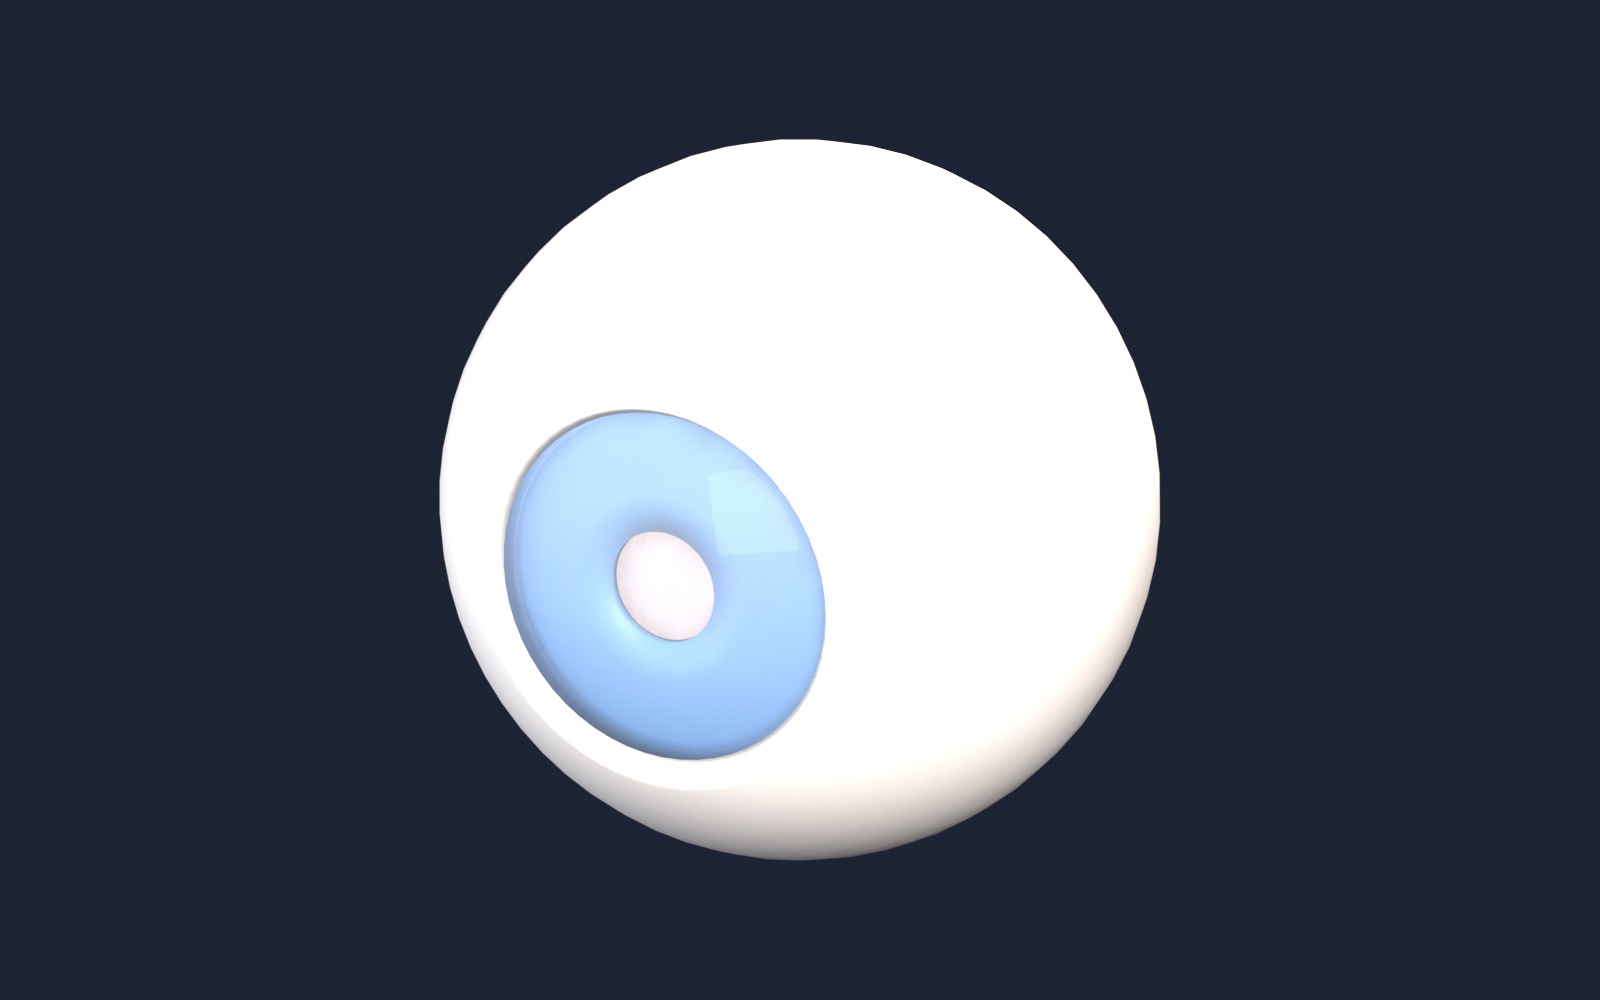
\includegraphics[width=\linewidth]{blender/01-completa.png}\caption{Completa}\end{subfigure}
\begin{subfigure}{0.32\textwidth}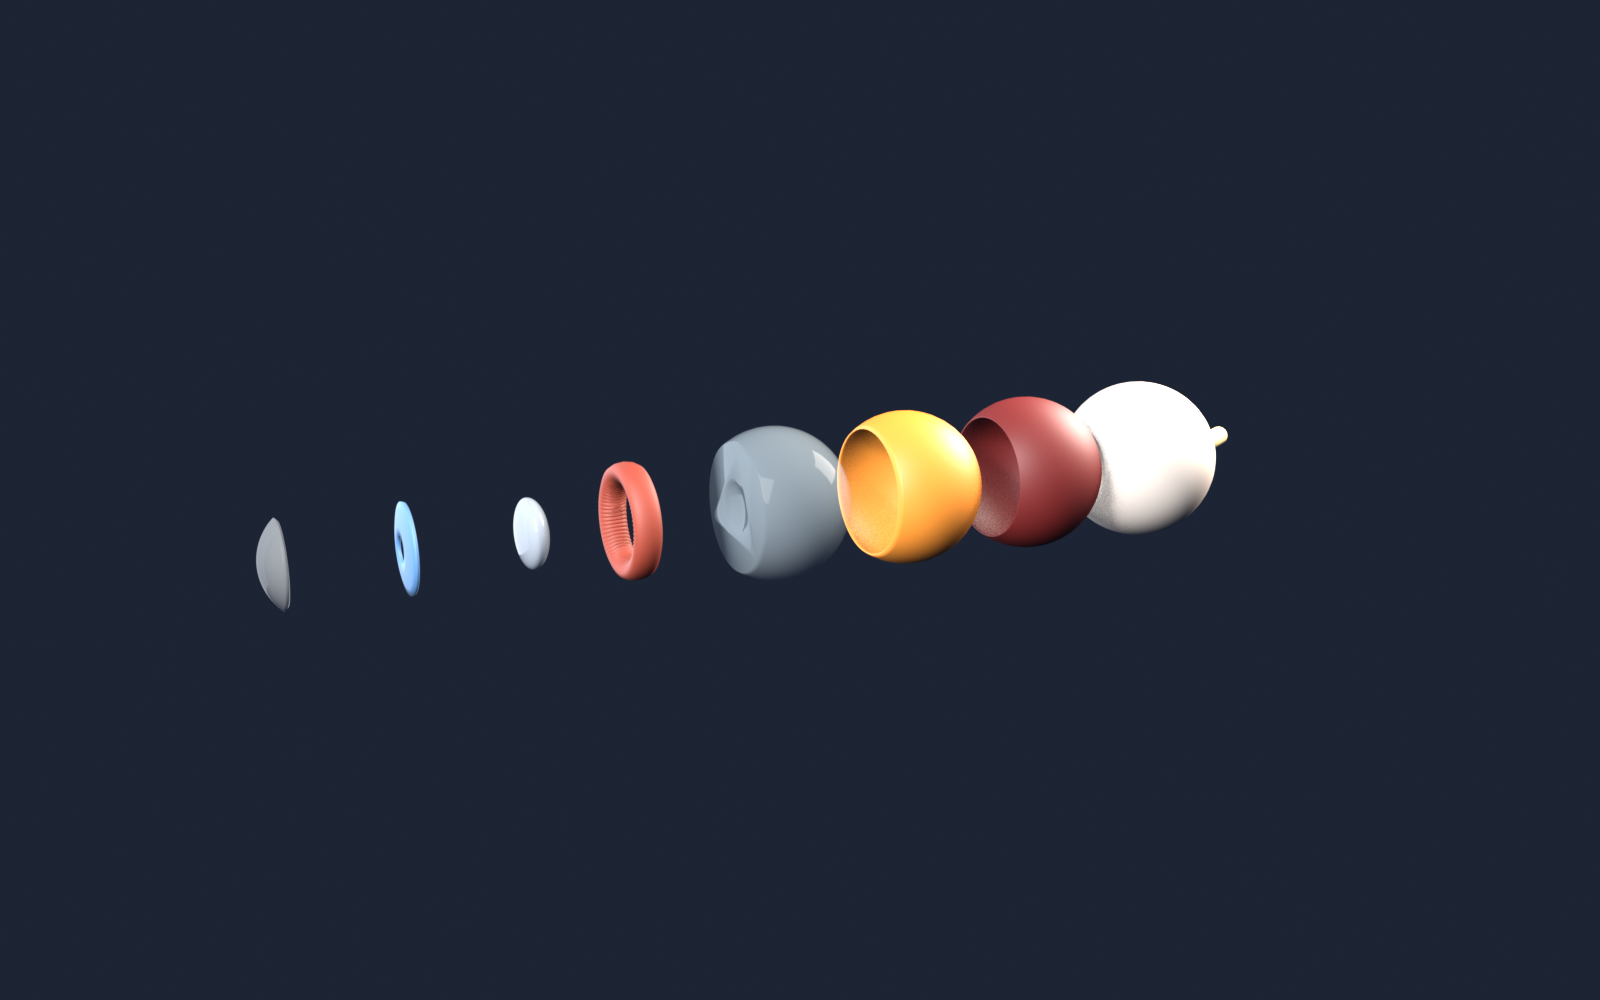
\includegraphics[width=\linewidth]{blender/02-desglosada.png}\caption{Desglosada}\end{subfigure}
\begin{subfigure}{0.32\textwidth}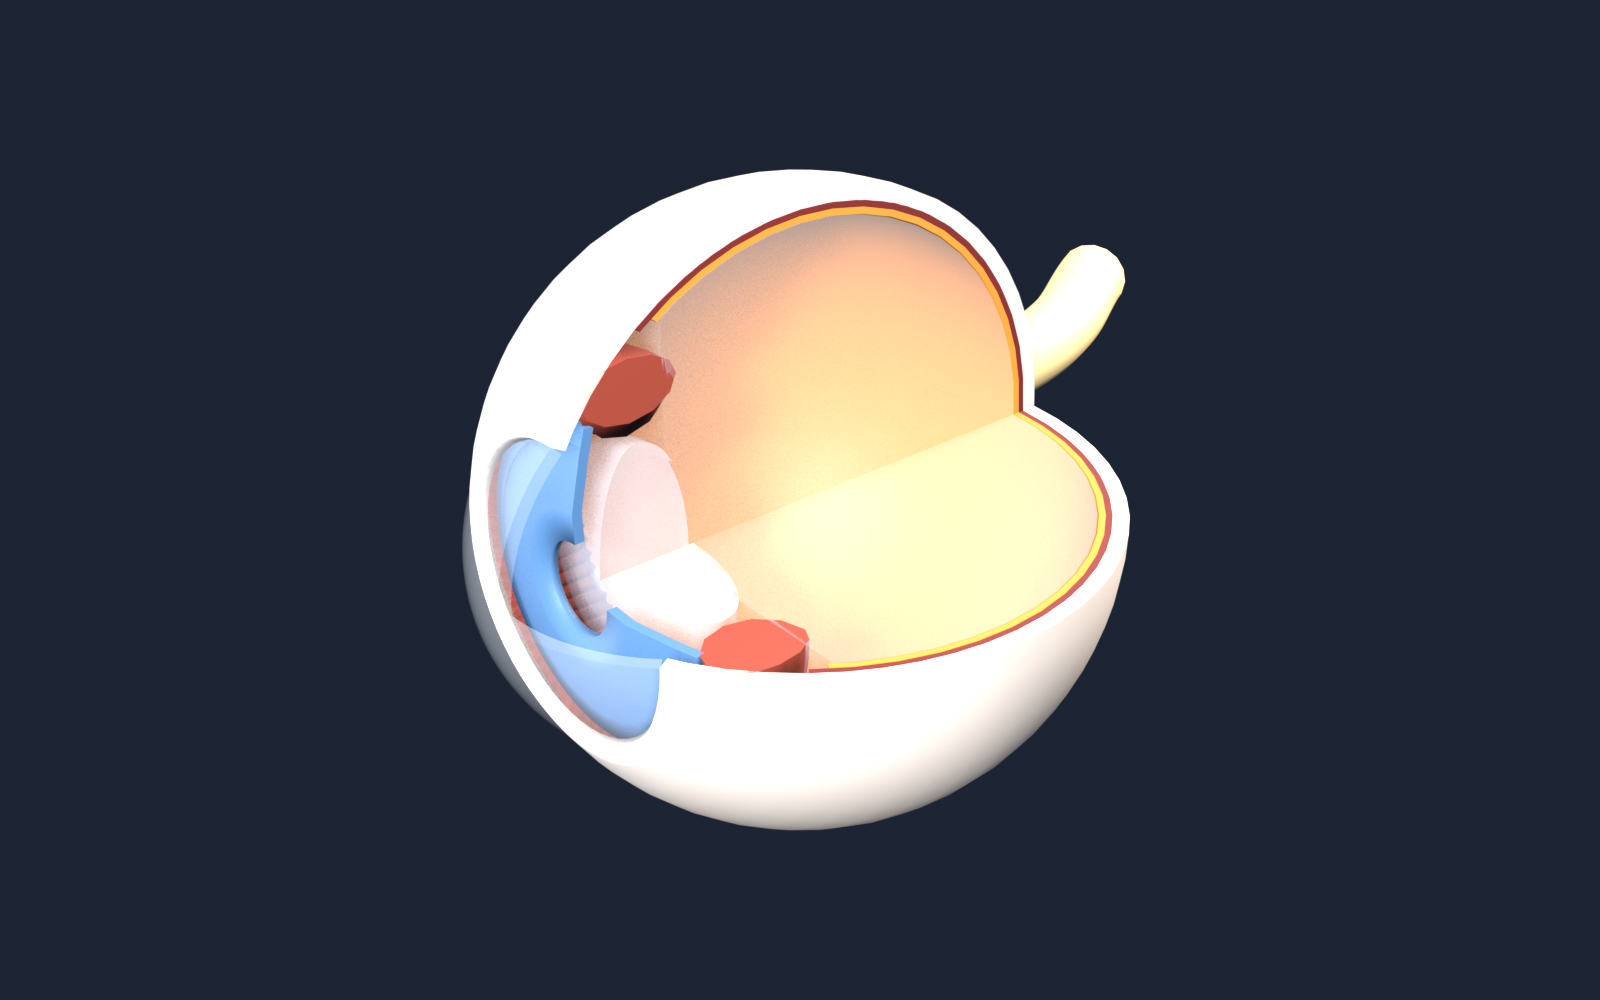
\includegraphics[width=\linewidth]{blender/03-corte.png}\caption{Corte}\end{subfigure}
\caption{Modelo base del ojo en Blender.}
\label{fig:blender}
\end{figure}

\subsection{Implementación en Unity}
Todo el código propio del atlas está en \texttt{Assets/Atlas/}. La Tabla~\ref{tab:scripts} resume sus componentes.

\begin{table}[H]
\centering
\small
\renewcommand{\arraystretch}{1.25}
\rowcolors{2}{gray!10}{white}
\begin{tabularx}{\textwidth}{>{\raggedright\arraybackslash}p{3.6cm} >{\raggedright\arraybackslash}X}
\toprule
\textbf{Componente} & \textbf{Función} \\
\midrule
\texttt{ParteAnatomica} & Datos de una pieza: nombre, término en kichwa, túnica, descripción, dato clave y distancia de separación. \\
\texttt{DatosOjo} & Contenido de las 9 piezas del ojo. \\
\texttt{OrganoController} & Vistas, separación de capas, selección, resaltado, colores por túnica y colocación frente al usuario. \\
\texttt{MenuAtlas} & Panel flotante construido por código; se usa con rayo o tocándolo con el dedo y se mueve agarrando su barra. \\
\texttt{ConstructorAtlas} & Herramienta de editor que genera materiales, prefab y escena. \\
\bottomrule
\end{tabularx}
\caption{Componentes del prototipo en Unity.}
\label{tab:scripts}
\end{table}

\subsection{Funcionalidades del prototipo}
Las capturas de esta sección se tomaron ejecutando la escena del atlas en modo \emph{Play} dentro de Unity. Como no se usó el visor, el fondo aparece en un color liso; en el Quest, en su lugar se ve el aula real.

\textbf{Vista completa.} El ojo aparece a unos 20\,cm de diámetro (unas ocho veces su tamaño real), en vista de tres cuartos. El estudiante lo agarra, lo gira y, con las dos manos, cambia su tamaño. El menú muestra los tres órganos; los pulmones y el riñón figuran como ``Próximamente''.

\begin{figure}[H]
\centering
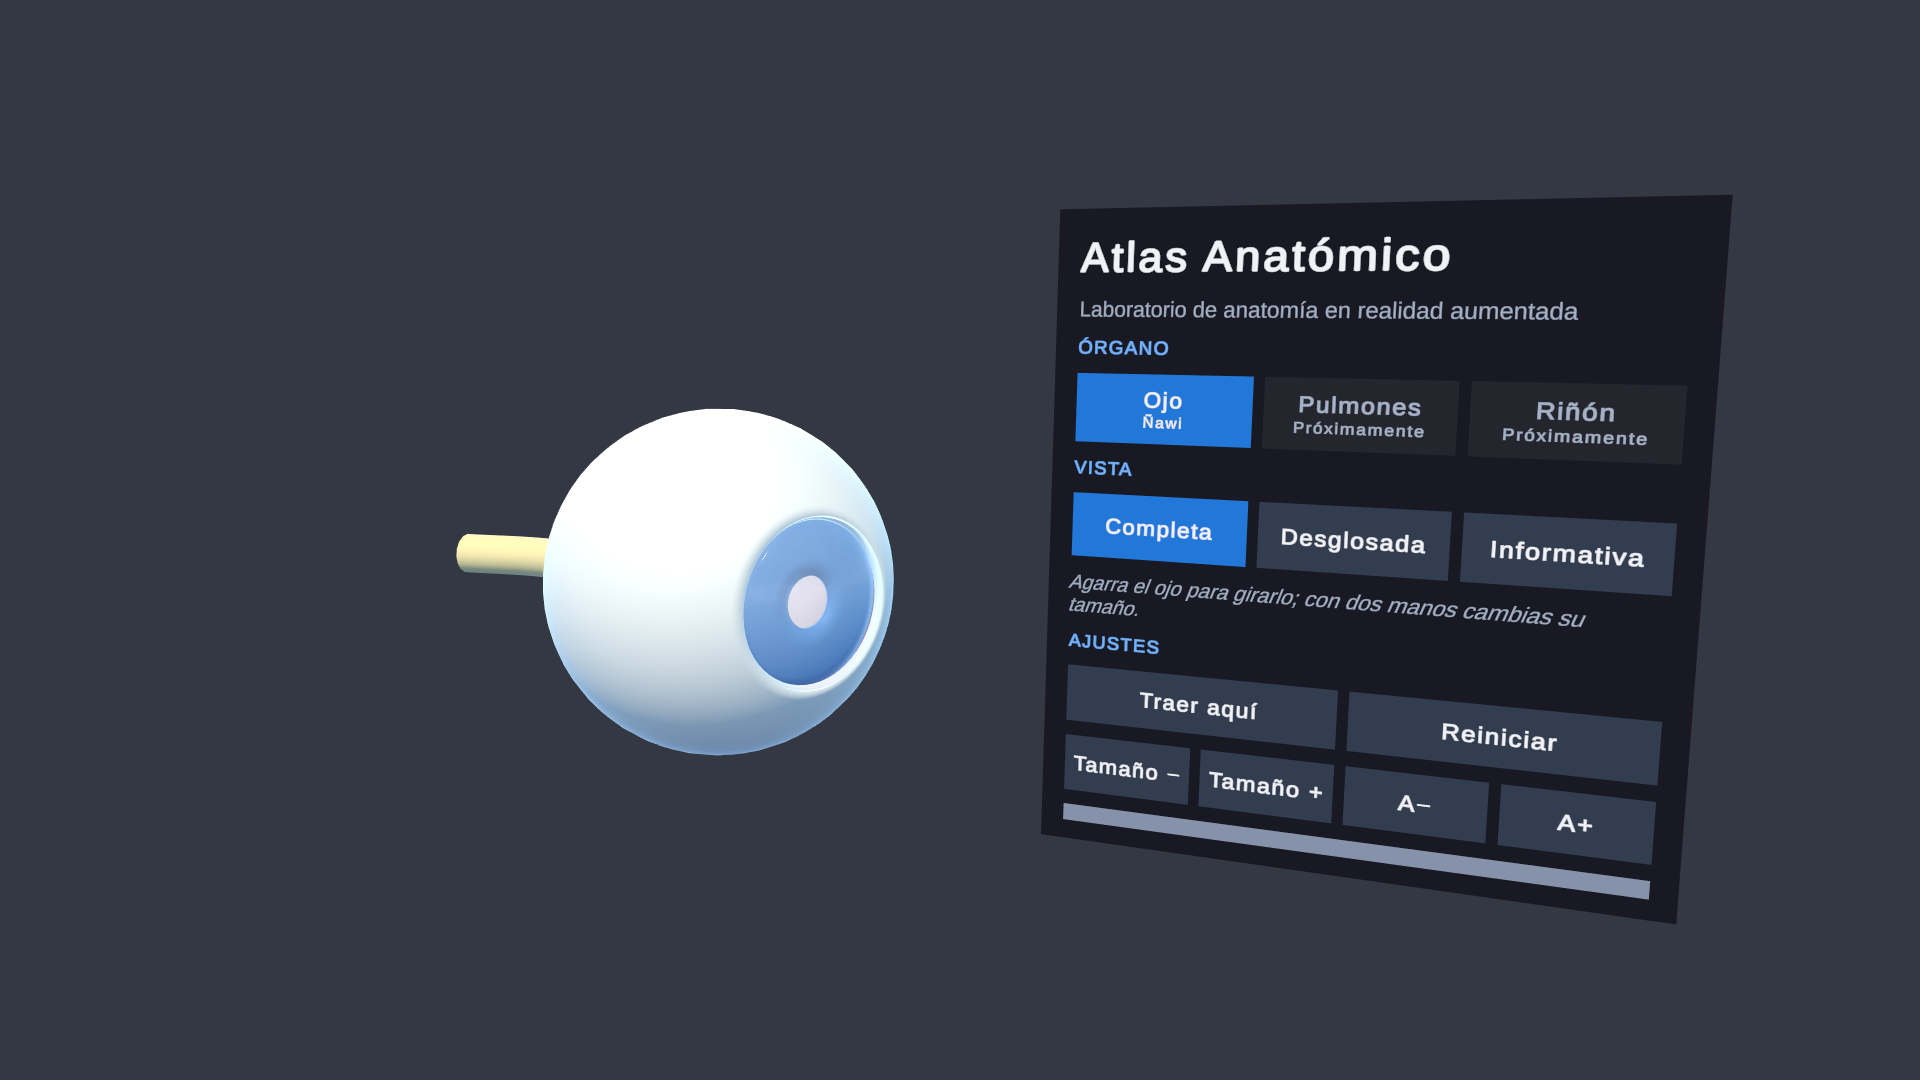
\includegraphics[width=0.85\textwidth]{capturas/01-vista-completa.png}
\caption{Vista completa del ojo junto al menú del atlas.}
\label{fig:completa}
\end{figure}

\textbf{Vista desglosada.} El ojo gira de lado y sus capas se separan a lo largo del eje óptico. Un deslizador controla la separación (de 0 a 1) y los botones \emph{Pieza anterior / siguiente} recorren las piezas una a una, lo que permite avanzar al ritmo de cada estudiante.

\begin{figure}[H]
\centering
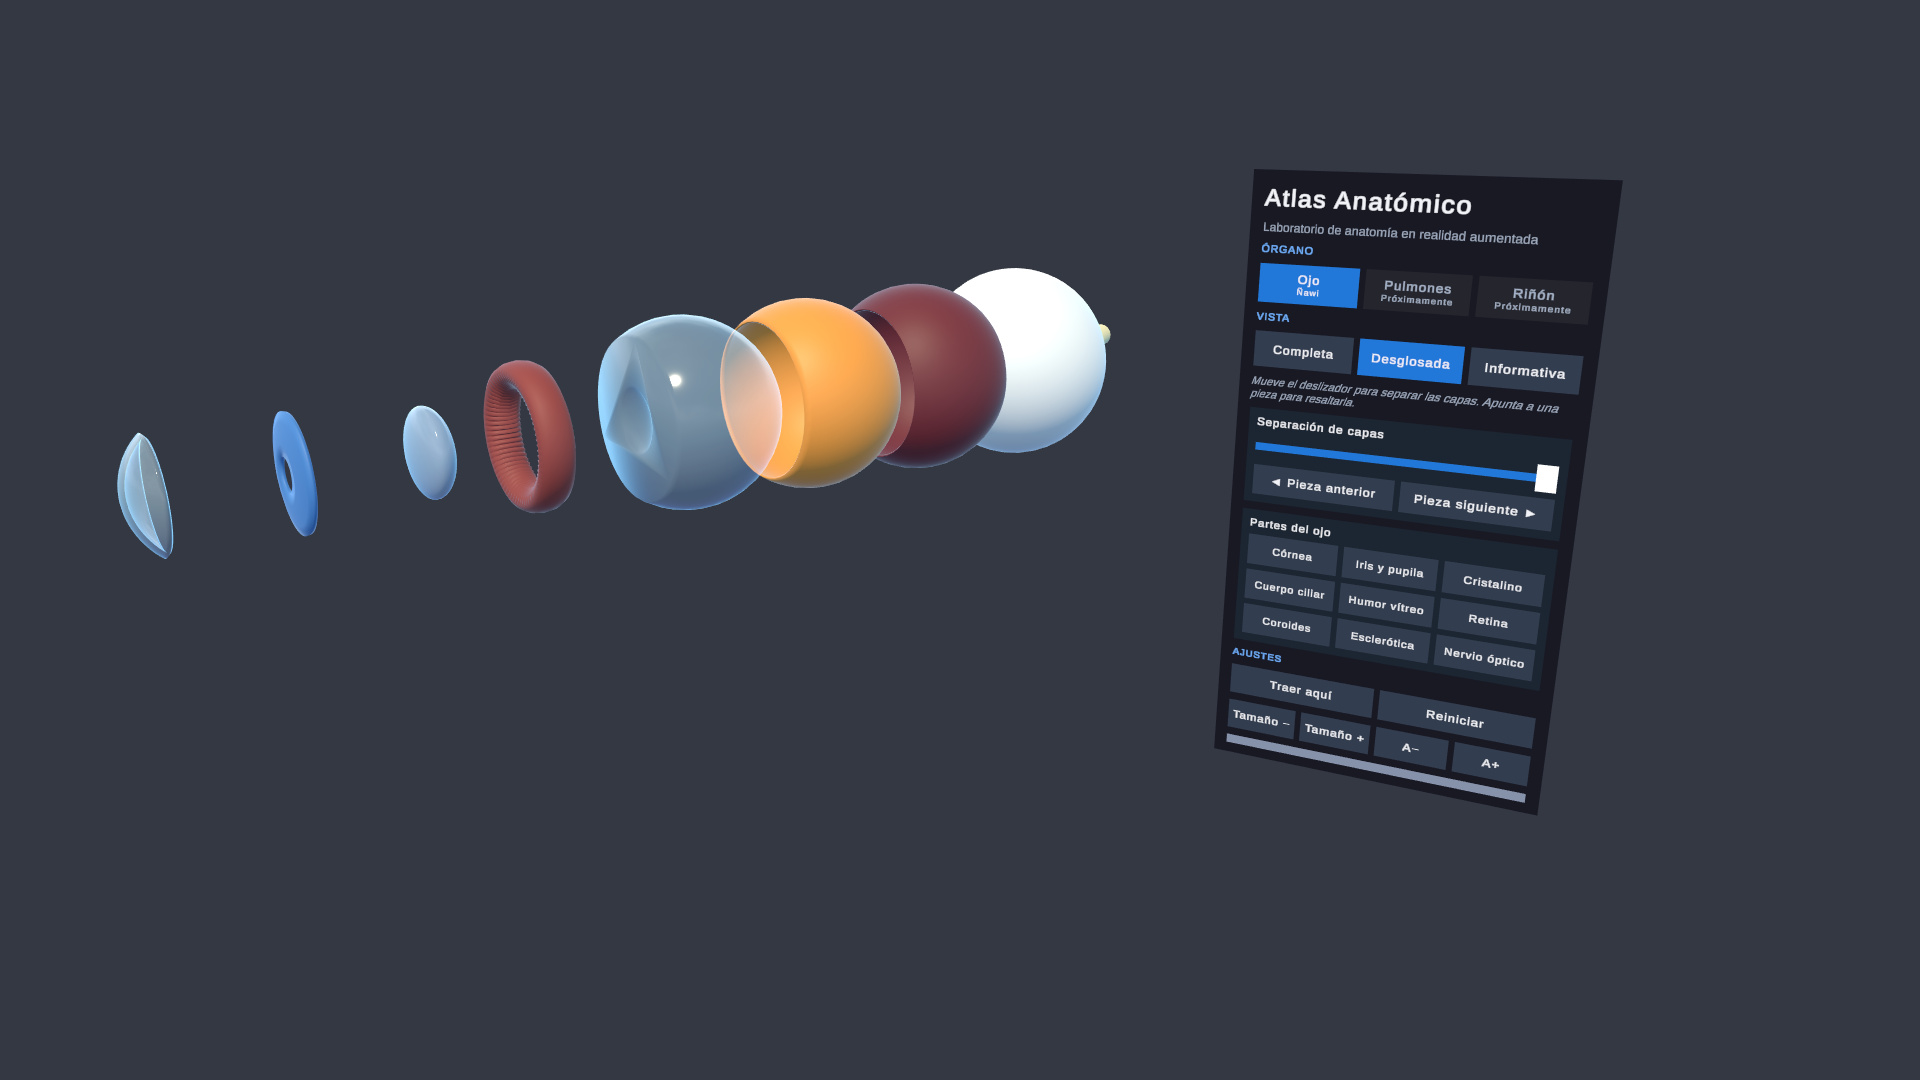
\includegraphics[width=0.85\textwidth]{capturas/02-vista-desglosada.png}
\caption{Vista desglosada con el deslizador de separación y los botones de las piezas.}
\label{fig:desglosada}
\end{figure}

\begin{figure}[H]
\centering
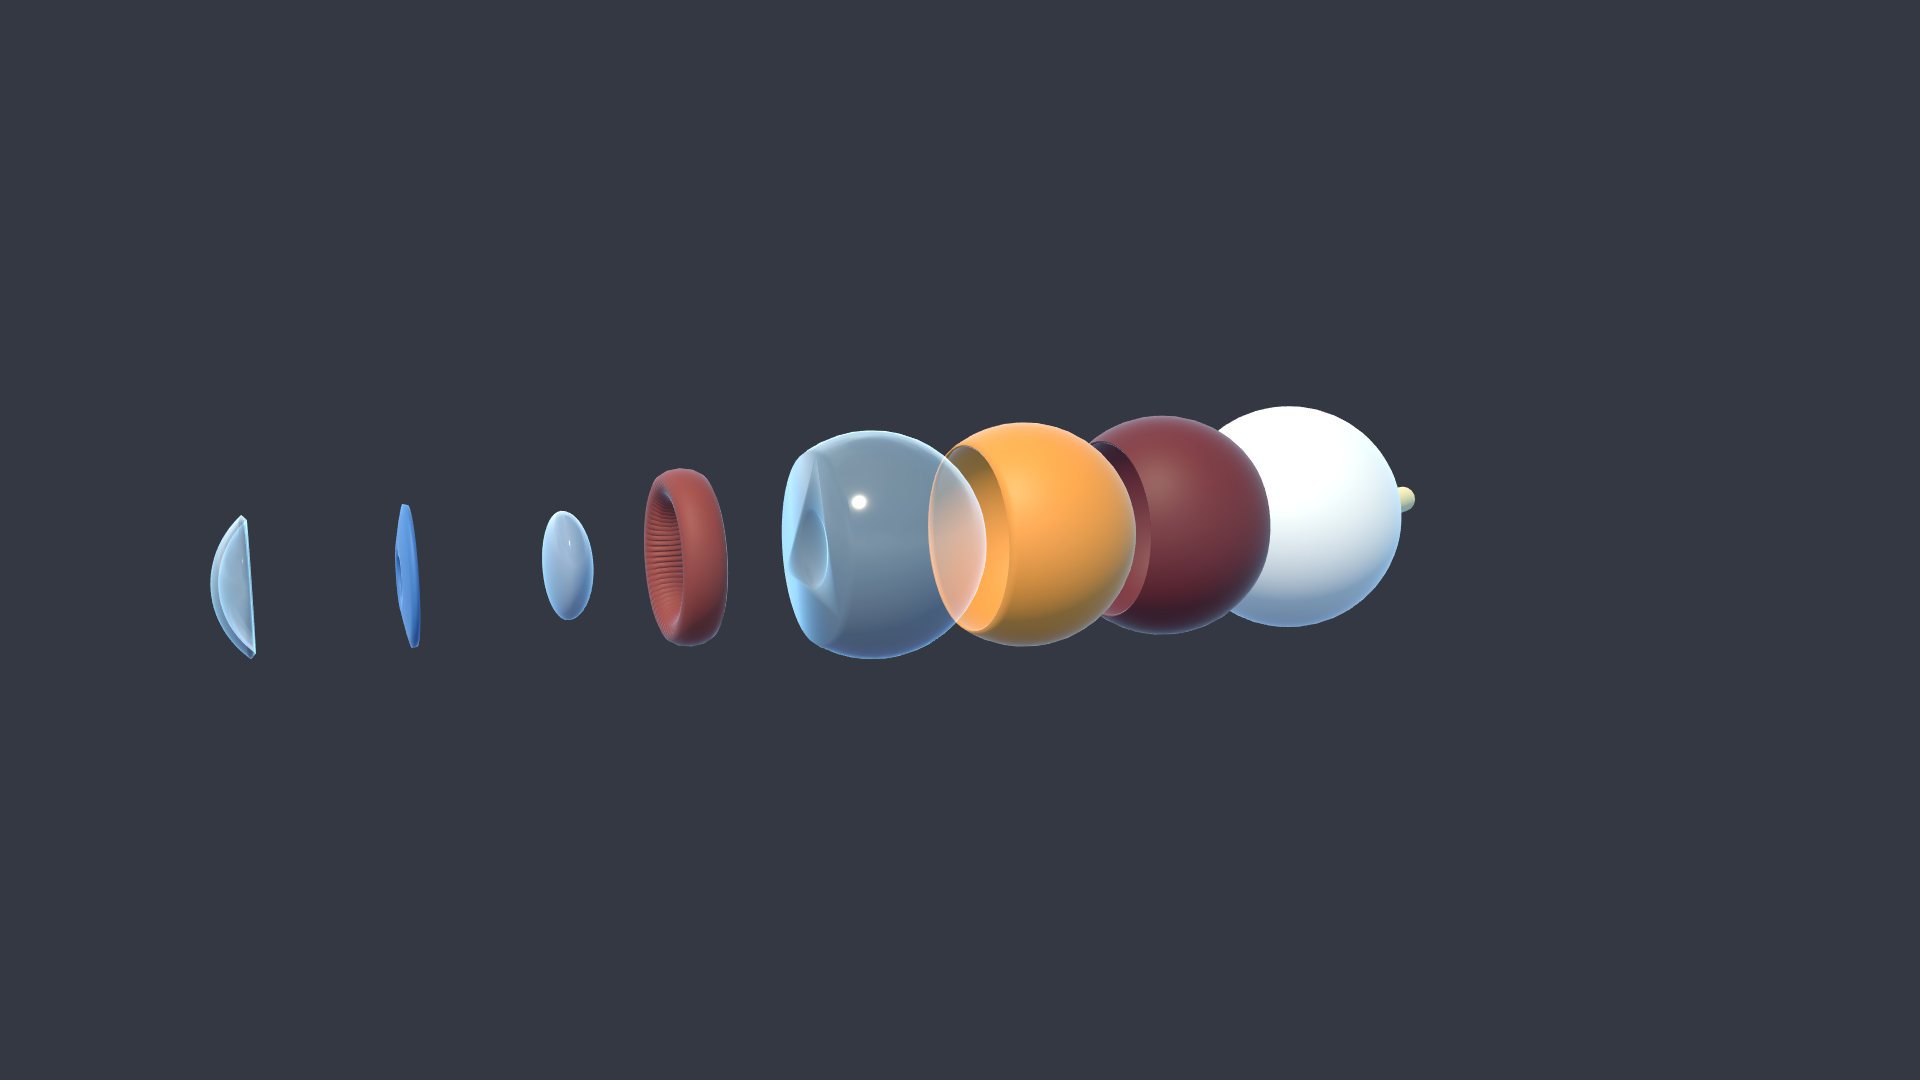
\includegraphics[width=0.85\textwidth]{capturas/03-detalle-desglosado.png}
\caption{Detalle de las 9 piezas separadas.}
\label{fig:detalle}
\end{figure}

\textbf{Vista informativa.} Al elegir una pieza, esta se resalta y las demás se vuelven transparentes. El panel muestra su nombre, el término en kichwa (o ``término por validar'' mientras no esté confirmado), la túnica a la que pertenece, una descripción breve y un dato clave.

\begin{figure}[H]
\centering
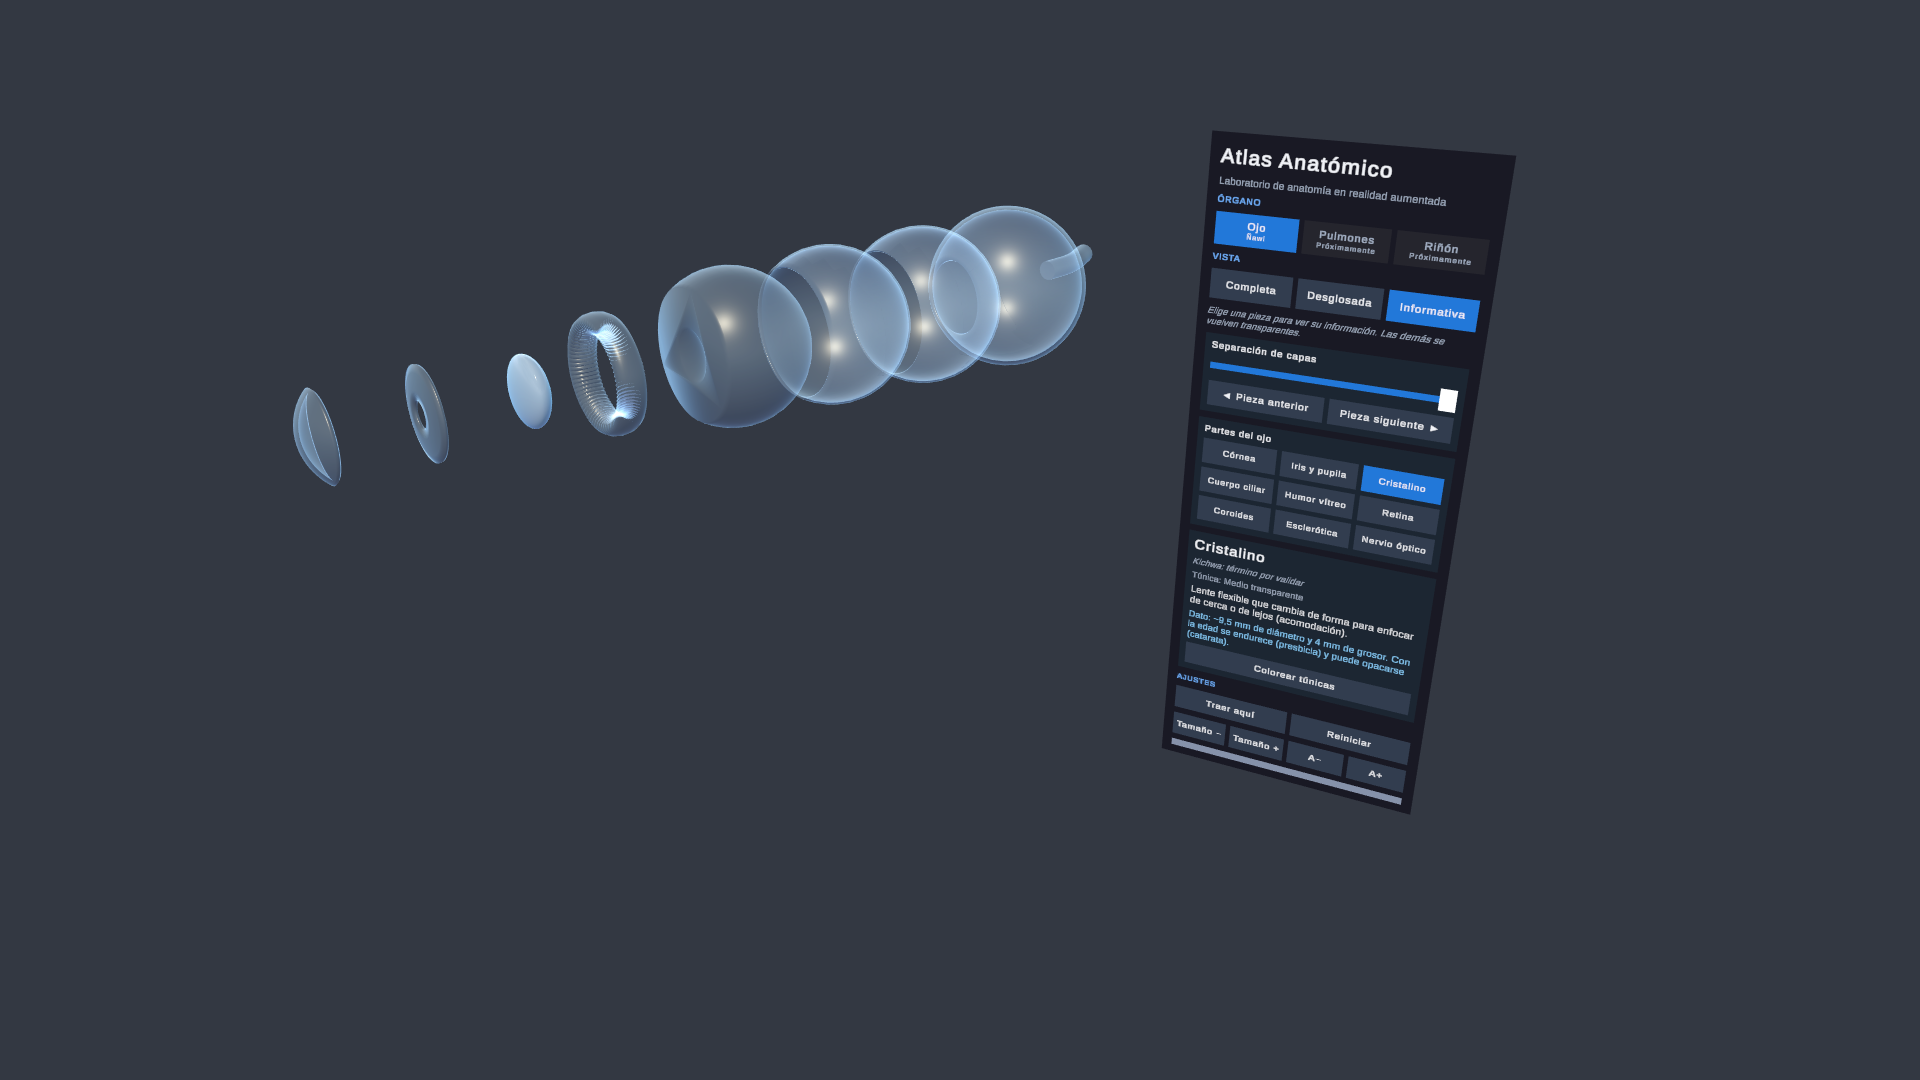
\includegraphics[width=0.85\textwidth]{capturas/04-vista-informativa.png}
\caption{Vista informativa con el cristalino seleccionado: la pieza se resalta y las demás se vuelven transparentes.}
\label{fig:informativa}
\end{figure}

\textbf{Colores por túnica.} El botón \emph{Colorear túnicas} agrupa las piezas en las tres túnicas del ojo: fibrosa (azul), vascular (rojo) y nerviosa (amarillo). Se eligieron colores de alto contraste entre sí y, en la vista informativa, el panel muestra una leyenda escrita y la túnica de la pieza elegida, de modo que la información no depende solo del color.

\begin{figure}[H]
\centering
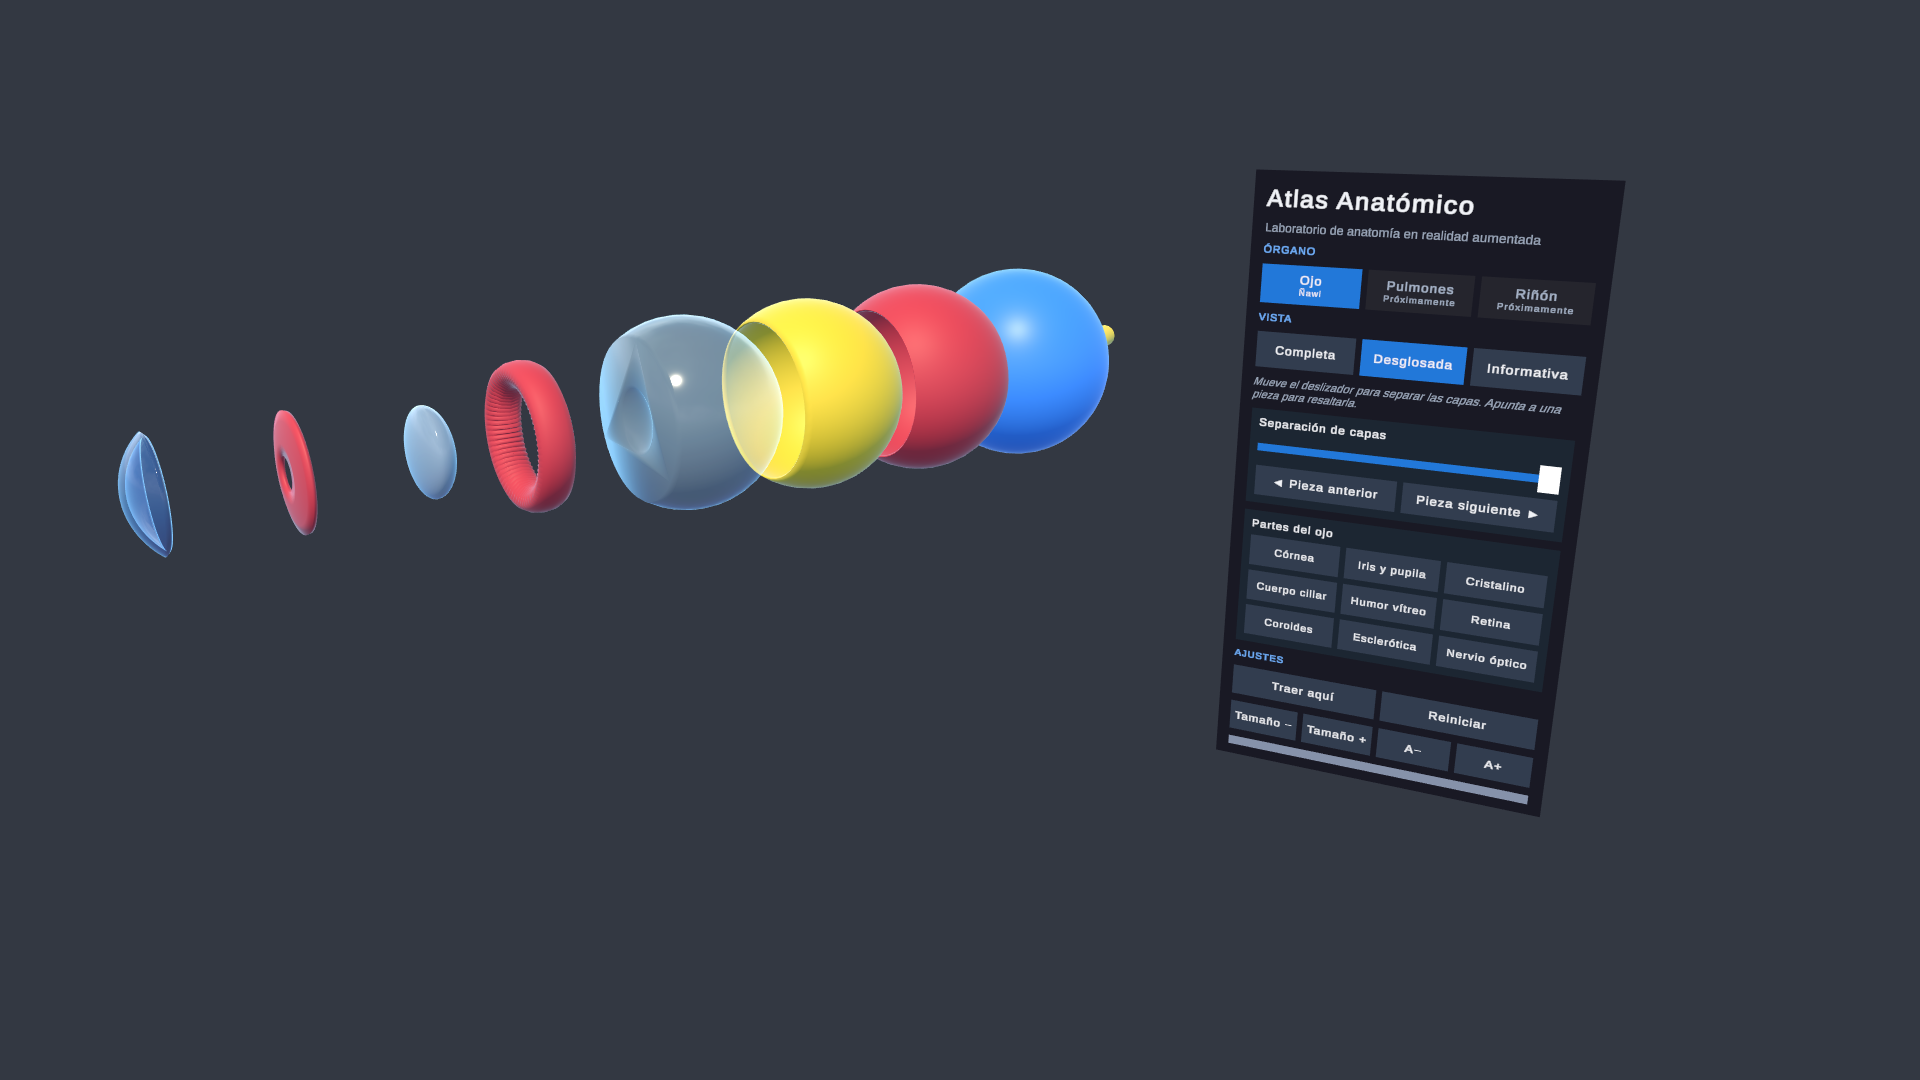
\includegraphics[width=0.85\textwidth]{capturas/05-tunicas.png}
\caption{Piezas coloreadas según su túnica.}
\label{fig:tunicas}
\end{figure}

\textbf{Panel y ajustes de accesibilidad.} La Figura~\ref{fig:paneles} muestra el panel de frente. Los botones \emph{A$-$ / A+} cambian el tamaño de todo el texto (entre 75\,\% y 180\,\%), \emph{Tamaño $-$ / +} escala el modelo, y \emph{Traer aquí} y \emph{Reiniciar} vuelven a colocar el órgano y el menú frente al estudiante sin que tenga que moverse. Con el texto ampliado (Figura~\ref{fig:paneles}b), las descripciones siguen siendo legibles, pero las etiquetas de algunos botones se parten en dos líneas; ajustar el ancho de los botones al tamaño del texto queda como mejora pendiente.

\begin{figure}[H]
\centering
\begin{subfigure}{0.40\textwidth}\centering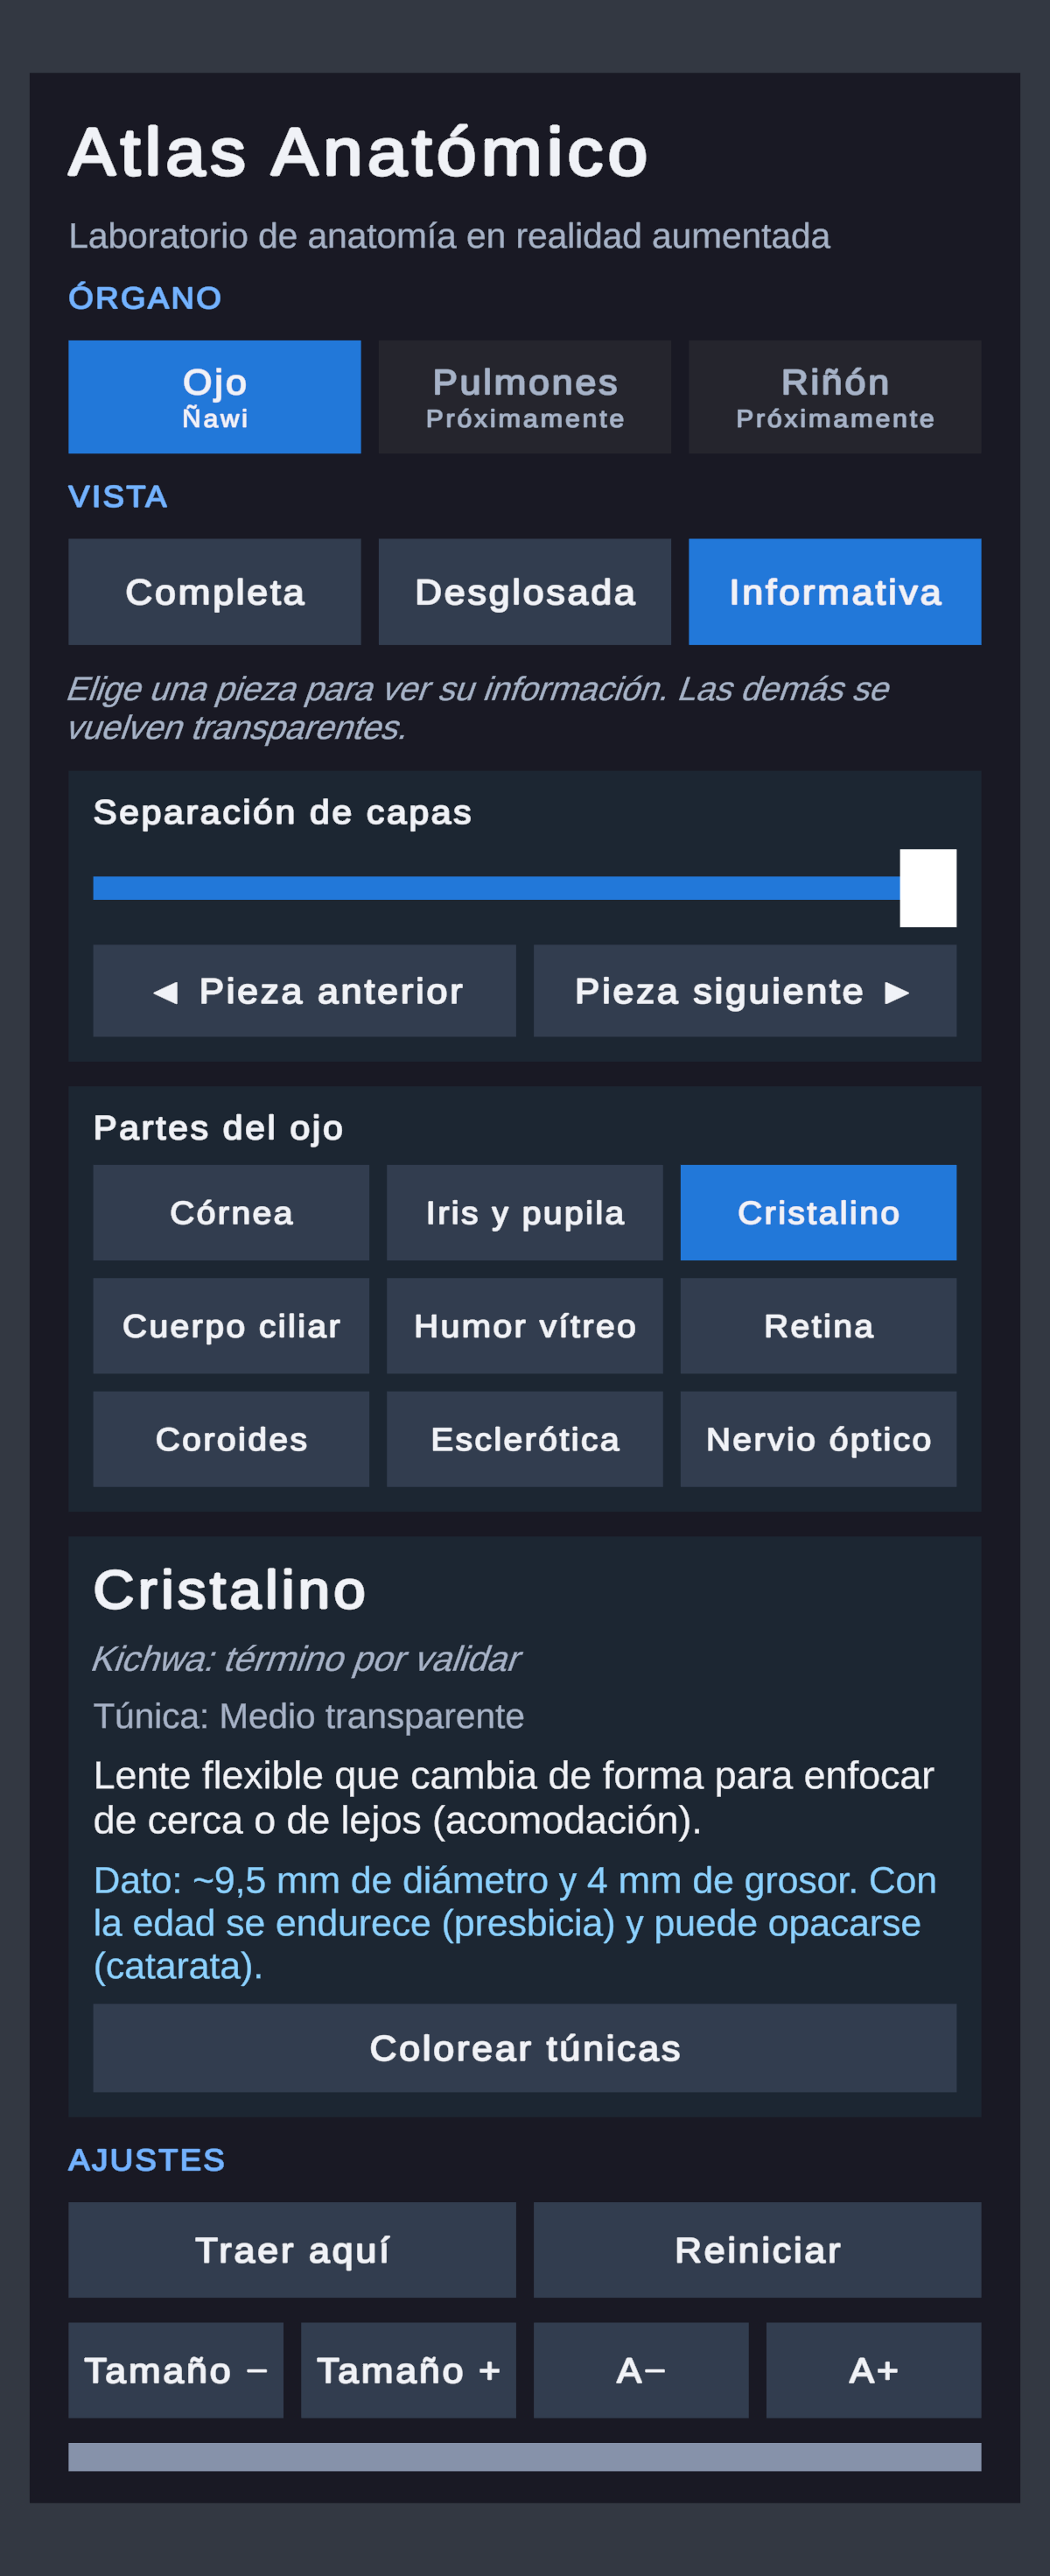
\includegraphics[height=10.5cm]{capturas/04b-panel-informativo.png}\caption{Texto normal, cristalino}\end{subfigure}
\hspace{0.5cm}
\begin{subfigure}{0.40\textwidth}\centering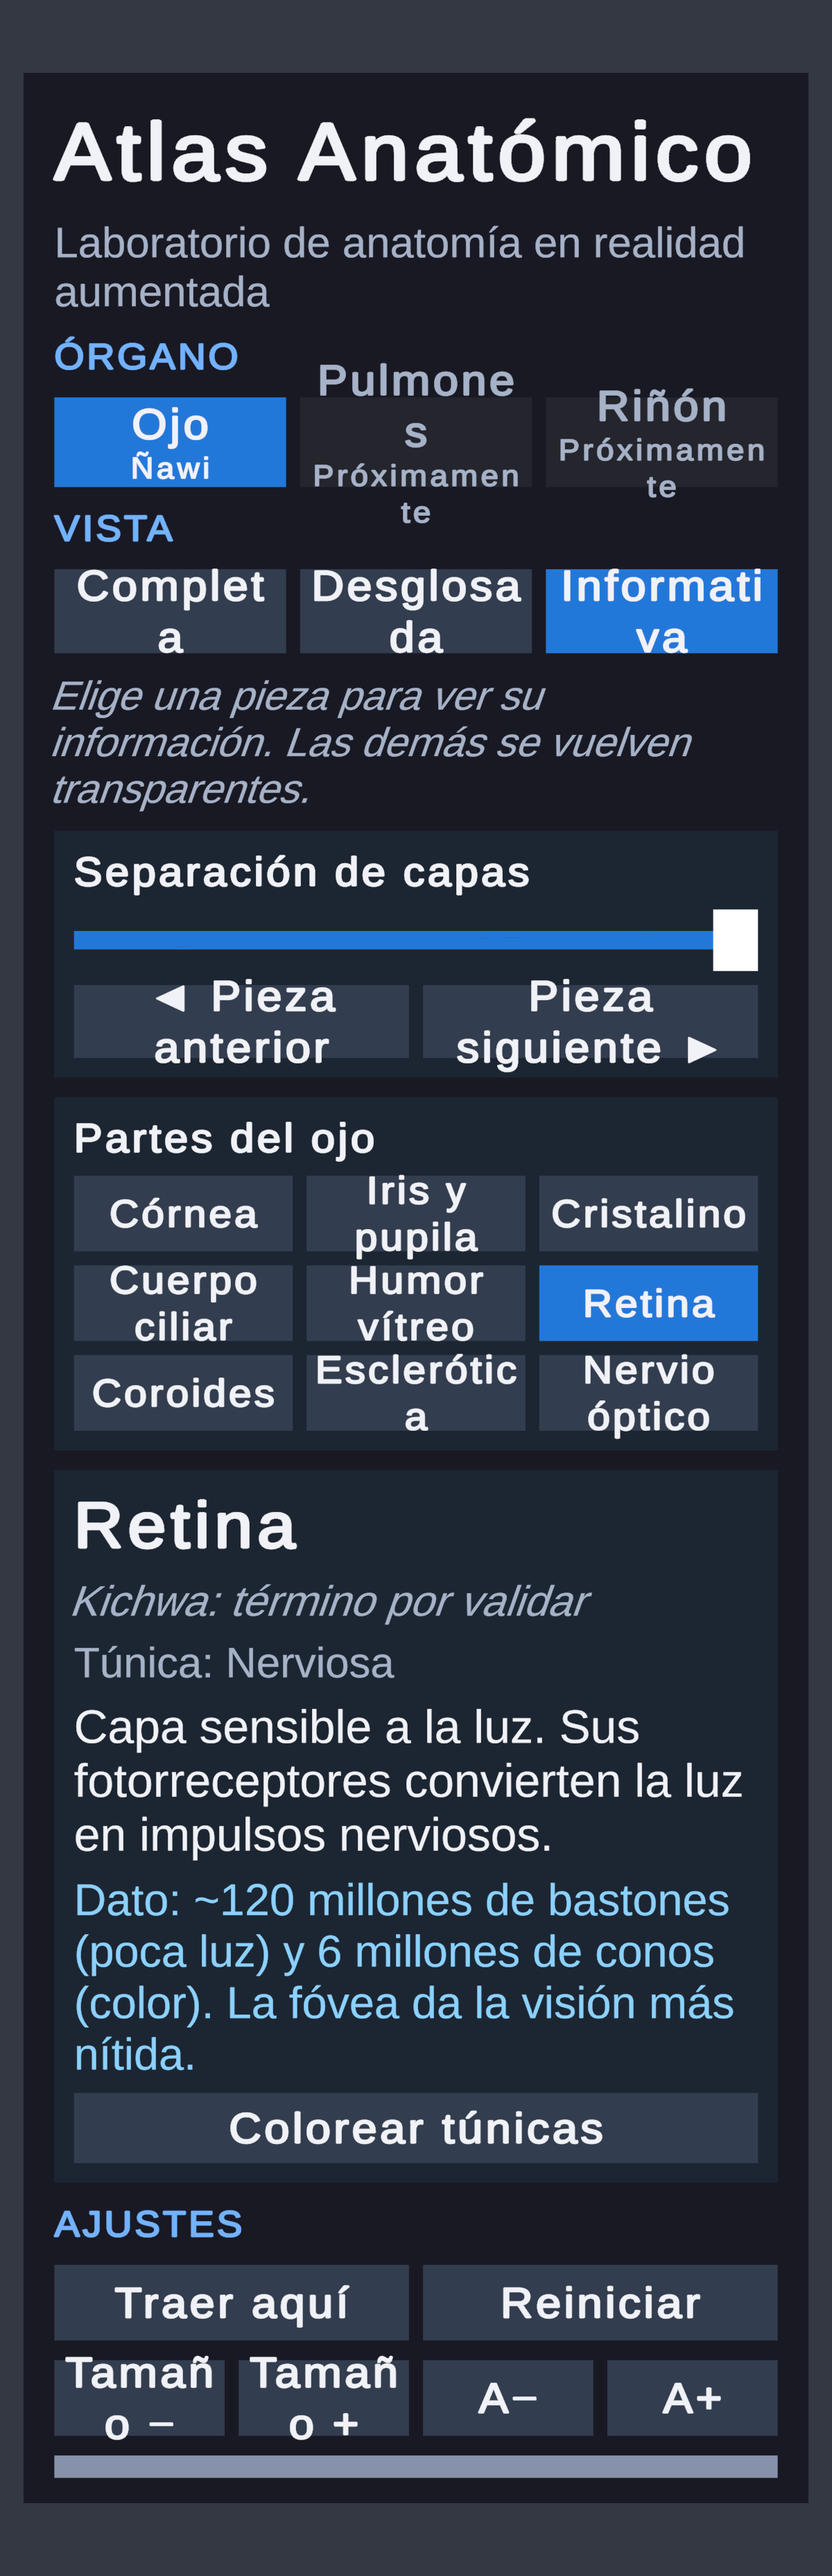
\includegraphics[height=10.5cm]{capturas/06-texto-ampliado.png}\caption{Texto ampliado (152\,\%), retina}\end{subfigure}
\caption{Panel del atlas en la vista informativa.}
\label{fig:paneles}
\end{figure}

% ============================================================
\section{Características inclusivas implementadas}
% ============================================================
\begin{description}
    \item[Lingüística e intercultural:] cada órgano y cada pieza tienen un campo para el término en kichwa. El nombre del órgano (\emph{ñawi}) ya aparece en el menú; los términos de las piezas se muestran como ``por validar'' en lugar de inventar traducciones, hasta confirmarlos con un hablante nativo y el diccionario oficial \cite{kichwa}.
    \item[Visual:] panel oscuro con texto claro (alto contraste), tamaño de texto ajustable, modelo escalable y resaltado de la pieza elegida con brillo y un pulso suave, no solo con color.
    \item[Auditiva:] la aplicación no transmite información solo por sonido; todo lo que se explica aparece escrito.
    \item[Motora:] se usa sentado y sin desplazarse; las piezas y los botones se seleccionan a distancia con un rayo (controles o seguimiento de manos) o tocándolos; los botones son grandes; el menú se puede mover y el órgano se recoloca con un solo botón.
    \item[Cognitiva:] cada vista muestra una frase de ayuda que explica qué hacer; los textos son cortos; el estudiante avanza pieza por pieza a su ritmo.
\end{description}

% ============================================================
\section{Pruebas realizadas}
% ============================================================
\begin{itemize}
    \item \textbf{Ejecución en el editor:} la escena se ejecutó en modo \emph{Play} de Unity 6. Una prueba automatizada (\texttt{PruebaCapturas}, del Test Framework de Unity) recorre las cinco situaciones mostradas en las figuras: vista completa, desglosada, informativa, colores por túnica y texto ampliado. Así se comprueba que el órgano y el menú responden correctamente, y de paso se generan las capturas del informe.
    \item \textbf{Rendimiento del modelo:} el ojo tiene unos 27\,000 triángulos, dentro del presupuesto de 30\,000 por órgano definido para el Quest. Las transparencias usan mezcla por alfa, sin refracción, para no penalizar al visor.
    \item \textbf{Pendiente:} compilar e instalar el prototipo en el Meta Quest 3 y aplicar el cuestionario SUS a al menos cinco usuarios, como se planteó en el Entregable~1.
\end{itemize}

% ============================================================
\section{Resultados y trabajo pendiente}
% ============================================================
\textbf{Resultados obtenidos:}
\begin{itemize}
    \item Grupo vulnerable seleccionado y necesidades definidas como requisitos verificables (Tabla~\ref{tab:necesidades}).
    \item Modelo 3D del ojo en 9 piezas, exportado y funcionando en Unity.
    \item Prototipo de realidad mixta con tres vistas, selección de piezas, colores por túnica y ajustes de accesibilidad.
    \item Flujo de trabajo Blender → Unity automatizado y documentado, listo para los demás órganos.
\end{itemize}

\textbf{Trabajo pendiente para los siguientes laboratorios:}
\begin{itemize}
    \item Modelar e integrar los pulmones (animación de respiración, Carlos Rivera) y el riñón (corte transversal, Samir Mideros); sus archivos de Blender ya están creados con la estructura y las convenciones del proyecto.
    \item Validar los términos en kichwa y migrarlos a Unity Localization con selector de idioma.
    \item Añadir narración por voz con subtítulos sincronizados.
    \item Hacer que los botones del panel se adapten al tamaño de texto ampliado.
    \item Colocar el órgano sobre una mesa detectada por el visor y hacer el corte por túnicas con plano de corte.
    \item Probar en el Quest 3 y evaluar la usabilidad con estudiantes.
\end{itemize}

% ============================================================
\section{Conclusiones}
% ============================================================
\begin{itemize}
    \item Definir las necesidades del grupo vulnerable antes de programar permitió convertir cada una en un requisito concreto y comprobar después si el prototipo la cumple.
    \item La realidad mixta resulta más inclusiva que la realidad virtual completa para este grupo: reduce el mareo, permite el uso sentado y mantiene al estudiante en contacto con su aula.
    \item Las funciones motoras, cognitivas y de baja visión ya están cubiertas en el prototipo; las necesidades lingüística y auditiva requieren aún la validación del kichwa y la narración con subtítulos.
    \item El flujo automatizado entre Blender y Unity reduce el trabajo para integrar los pulmones y el riñón en los próximos laboratorios.
\end{itemize}

% ============================================================
\section{Bibliografía}
% ============================================================
\begingroup
\renewcommand{\section}[2]{}
\begin{thebibliography}{9}
\bibitem{moro2017} Moro, C., Štromberga, Z., Raikos, A. y Stirling, A. (2017). The effectiveness of virtual and augmented reality in health sciences and medical anatomy. \emph{Anatomical Sciences Education}, 10(6), 549--559.
\bibitem{bodyparts3d} Mitsuhashi, N., Fujieda, K., Tamura, T., Kawamoto, S., Takagi, T. y Okubo, K. (2009). BodyParts3D: 3D structure database for anatomical concepts. \emph{Nucleic Acids Research}, 37, D782--D785.
\bibitem{wcag22} World Wide Web Consortium (W3C). (2023). \emph{Web Content Accessibility Guidelines (WCAG) 2.2}. \url{https://www.w3.org/TR/WCAG22/}
\bibitem{iso9241} International Organization for Standardization. (2019). \emph{ISO 9241-210:2019. Ergonomics of human-system interaction -- Part 210: Human-centred design for interactive systems}.
\bibitem{unityxr} Unity Technologies. (2026). \emph{XR Interaction Toolkit documentation}. \url{https://docs.unity3d.com/Packages/com.unity.xr.interaction.toolkit@latest}
\bibitem{arfoundation} Unity Technologies. (2026). \emph{AR Foundation documentation}. \url{https://docs.unity3d.com/Packages/com.unity.xr.arfoundation@latest}
\bibitem{blender} Blender Foundation. (2026). \emph{Blender Reference Manual}. \url{https://docs.blender.org/manual/es/latest/}
\bibitem{kichwa} Ministerio de Educación del Ecuador. (2009). \emph{Kichwa Yachakukkunapak Shimiyuk Kamu: diccionario kichwa--castellano}. Quito: DINEIB.
\bibitem{constitucion} Asamblea Constituyente. (2008). \emph{Constitución de la República del Ecuador}, art. 1 y art. 2.
\end{thebibliography}
\endgroup

\end{document}
